\documentclass[11pt,letterpaper]{article}

\usepackage[utf8]{inputenc}
\usepackage[T1]{fontenc}
\usepackage[spanish,es-noshorthands]{babel}
\usepackage[margin=2.5cm]{geometry}
\usepackage{graphicx}
\usepackage{float}
\usepackage{booktabs}
\usepackage{hyperref}

\graphicspath{{../pruebas/graficas/}{.}}

\begin{document}

%========================= PORTADA =========================
\begin{titlepage}
\centering

{\bfseries UNIVERSIDAD DEL VALLE DE GUATEMALA}\\[0.3em]
CC3067 - Redes\\[0.2em]
Sección 10\\[0.2em]
Ing. Jorge Yass\\[2.5em]


\includegraphics[width=0.32\textwidth]{Uvg_logo.jpg}\\[2.5em]

{\LARGE Laboratorio \#2: Esquemas de\\[0.4em] detección y corrección de\\[0.4em] errores}\\[2em]

{\large Reporte grupal}\\[2em]

Fernando Andree Hernández Martínez \quad 23645\\[0.3em]
Fernando José Rueda Rodas \quad 23748\\[2em]

\vfill

{\bfseries GUATEMALA}\\[0.2em]
{\bfseries 2 de agosto de 2026}

\end{titlepage}

%========================= DESCRIPCIÓN =========================
\section{Descripción de la práctica}

% TODO: revisar/ampliar esta descripción.
En esta práctica se implementó una arquitectura de capas (Aplicación,
Presentación, Enlace, Ruido y Transmisión) para la comunicación entre un cajero
automático (emisor, en Python) y el servidor de una entidad financiera
(receptor, en Node.js), a través de un canal no confiable simulado. En la capa
de Enlace se integraron dos algoritmos: \textbf{Hamming (12,8)} para corrección
de errores y \textbf{CRC-32} (polinomio estándar IEEE 802.3, $0x04C11DB7$) para
detección de errores. El ruido se simula volteando cada bit de la trama con una
probabilidad configurable, y la transmisión se realiza mediante sockets TCP con
mensajes JSON delimitados por salto de línea, lo que permite la
interoperabilidad entre ambos lenguajes.

\section{Metodología de pruebas}

% TODO: ajustar si cambian los parámetros del benchmark.
Las pruebas se automatizaron con un \emph{harness} (\texttt{pruebas/benchmark.py})
que ejecuta la arquitectura completa de extremo a extremo: por cada envío se
genera un mensaje aleatorio, se codifica, se calcula la integridad, se aplica
ruido y se transmite por sockets al receptor en Node, clasificando la respuesta
del banco en tres resultados posibles:

\begin{itemize}
  \item \textbf{Éxito}: el mensaje entregado coincide con el original.
  \item \textbf{Error detectado}: el algoritmo detectó errores que no pudo
        (o no puede) corregir y el mensaje fue rechazado.
  \item \textbf{Error no detectado}: el banco aceptó un mensaje corrupto.
\end{itemize}

Se probaron todas las combinaciones de: algoritmo (Hamming, CRC-32), tamaño de
mensaje (4, 16, 64 y 256 caracteres) y probabilidad de error por bit
($10^{-3}$ a $10^{-1}$), con 200 repeticiones por combinación
(11\,200 envíos en total, semilla fija para reproducibilidad).

%========================= RESULTADOS =========================
\section{Resultados}

\begin{figure}[H]
  \centering
  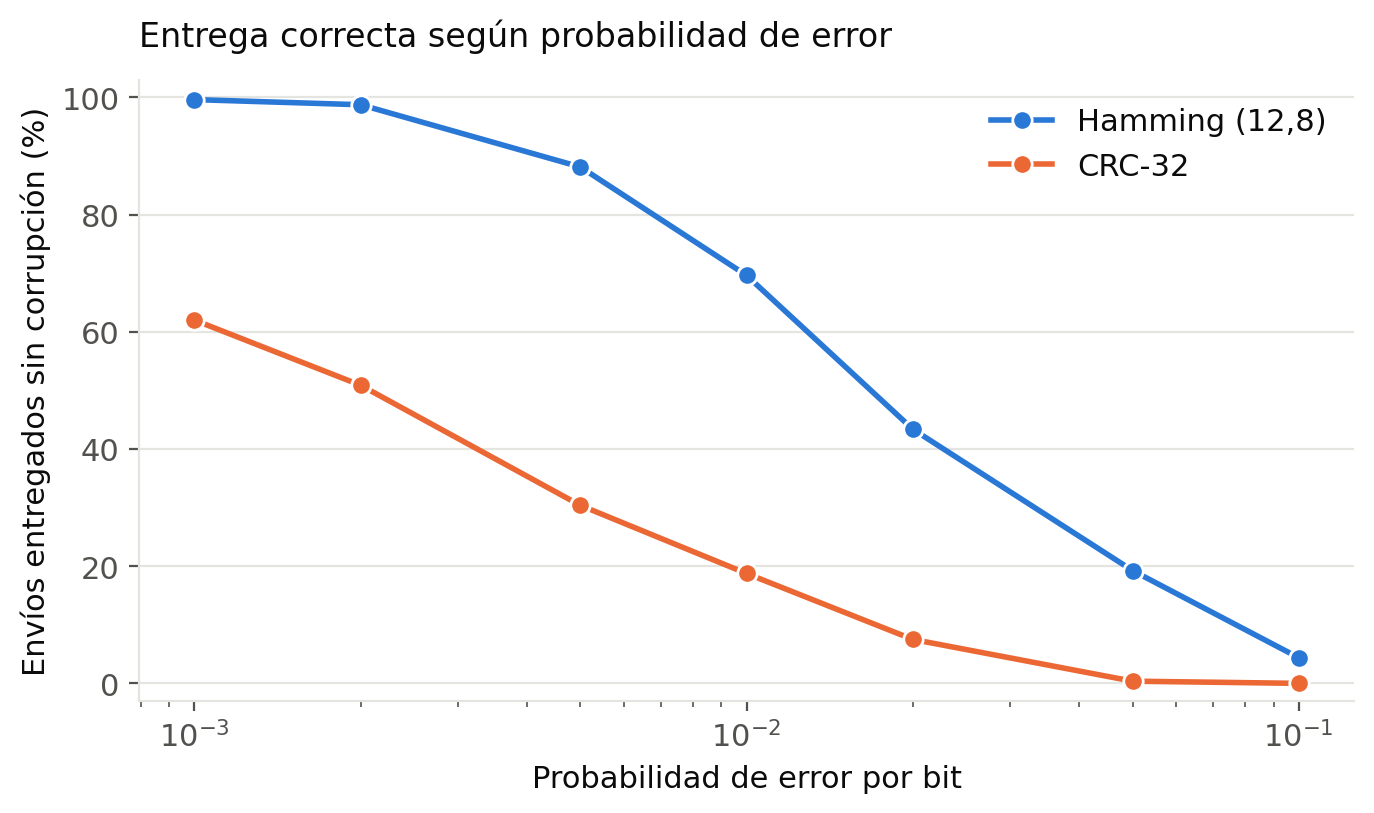
\includegraphics[width=0.85\textwidth]{exito_vs_tasa.png}
  \caption{Porcentaje de envíos entregados sin corrupción según la probabilidad
  de error por bit. Hamming mantiene la entrega gracias a la corrección;
  CRC-32 solo entrega tramas que llegaron intactas.}
  \label{fig:exito}
\end{figure}

\begin{figure}[H]
  \centering
  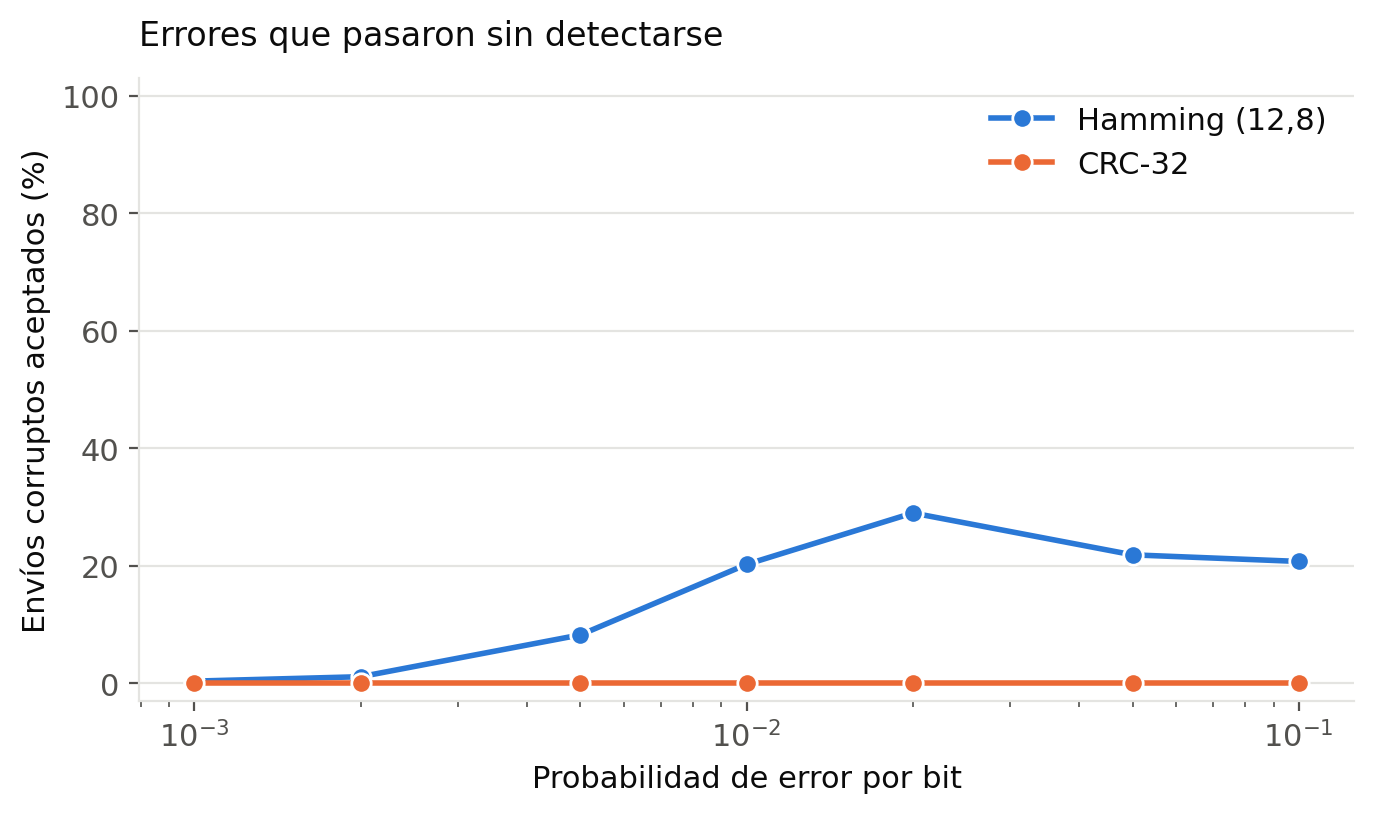
\includegraphics[width=0.85\textwidth]{no_detectados_vs_tasa.png}
  \caption{Porcentaje de envíos corruptos aceptados como válidos. CRC-32 no
  dejó pasar ningún error en las pruebas; Hamming ``corrige mal'' cuando hay
  más de un error por bloque.}
  \label{fig:nodetectados}
\end{figure}

\begin{figure}[H]
  \centering
  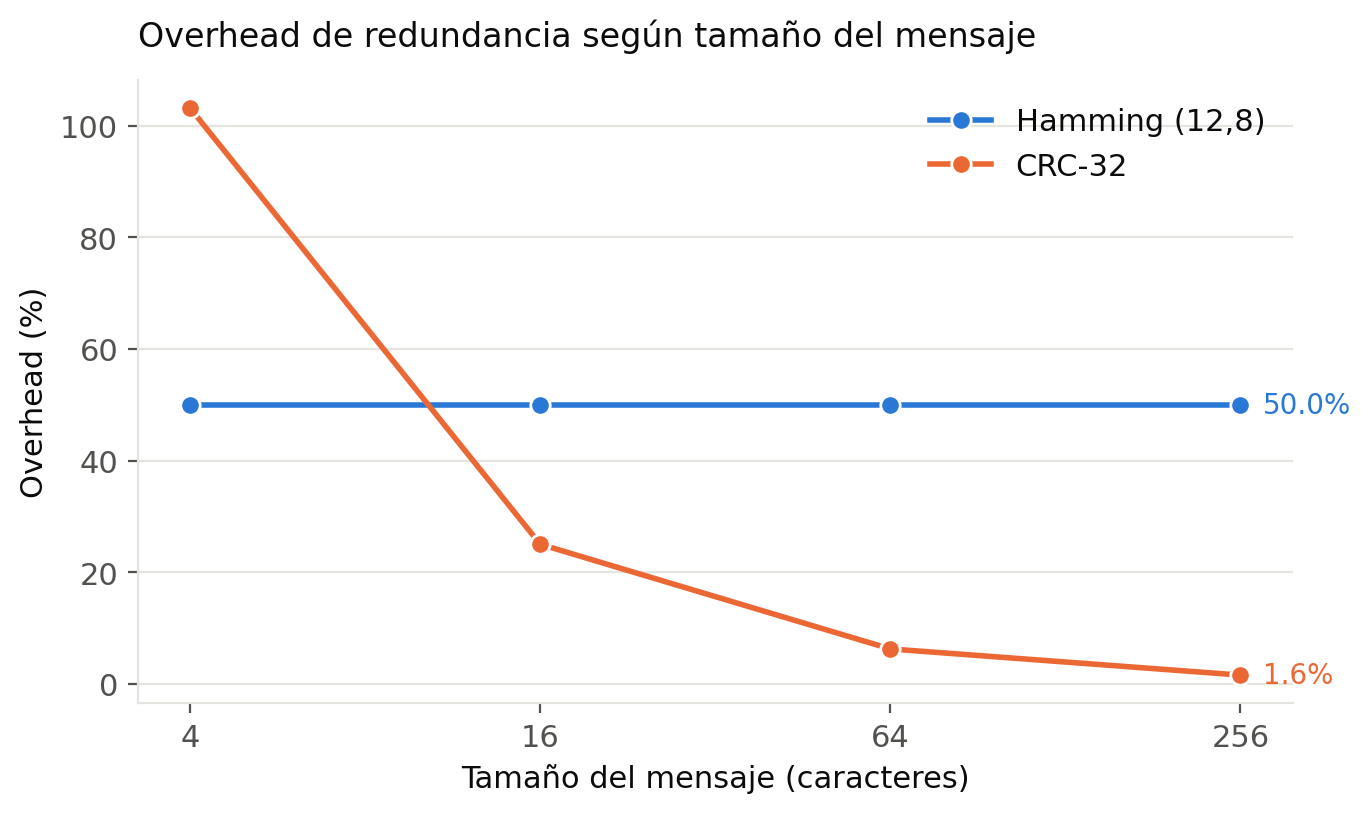
\includegraphics[width=0.85\textwidth]{overhead_vs_tamano.png}
  \caption{Overhead de redundancia según el tamaño del mensaje. Hamming (12,8)
  agrega un 50\% constante; el CRC-32 fijo de 32 bits se diluye al crecer el
  mensaje.}
  \label{fig:overhead}
\end{figure}

\begin{figure}[H]
  \centering
  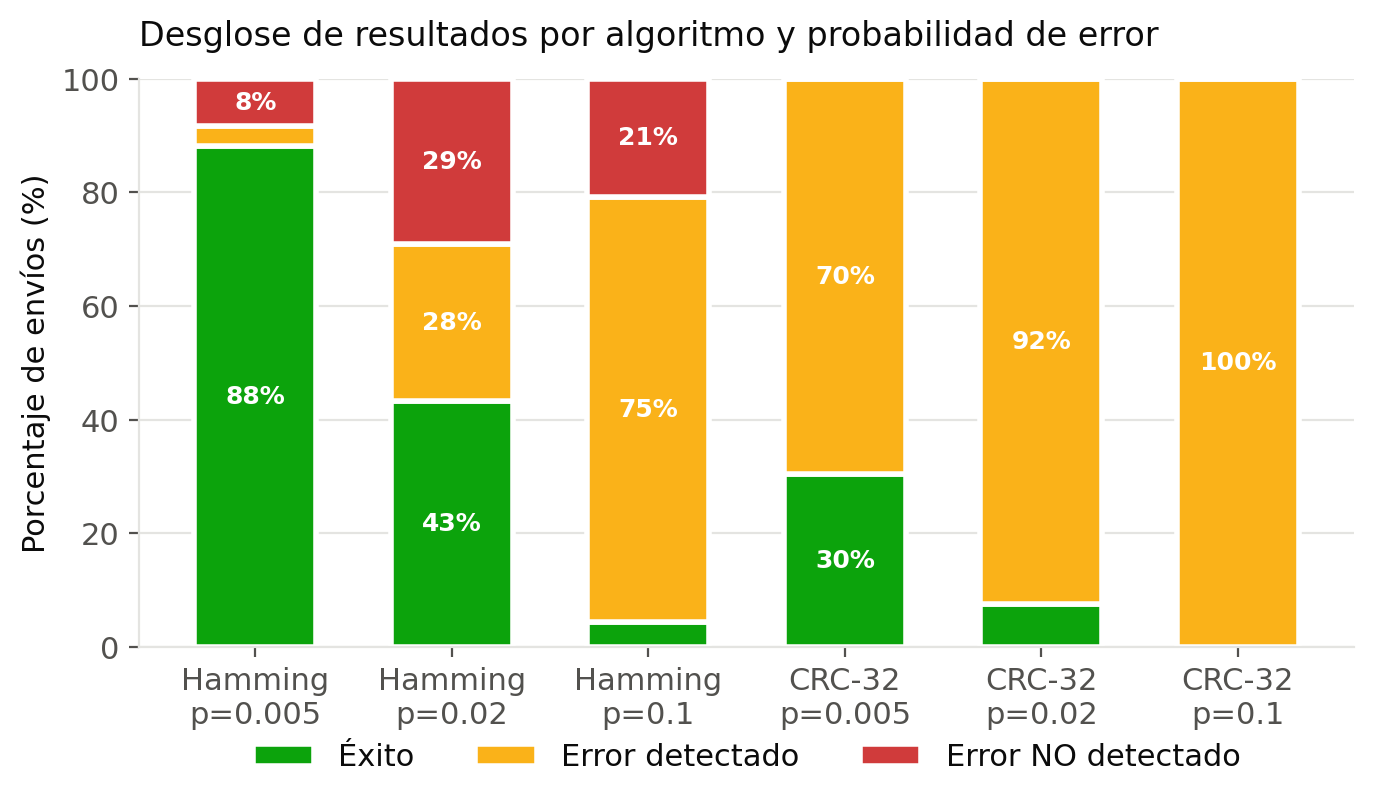
\includegraphics[width=0.85\textwidth]{desglose_resultados.png}
  \caption{Desglose de resultados por algoritmo para tres probabilidades de
  error representativas.}
  \label{fig:desglose}
\end{figure}

%========================= DISCUSIÓN =========================
\section{Discusión}

% TODO: desarrollar la discusión con base en las figuras.
% Preguntas guía del laboratorio:
%  - ¿Qué algoritmo tuvo un mejor funcionamiento?
%  - ¿Qué algoritmo es más flexible para aceptar mayores tasas de errores?
%  - ¿Cuándo es mejor usar detección en lugar de corrección?

%========================= COMENTARIO GRUPAL (opcional) =========================
% \section{Comentario grupal}

%========================= CONCLUSIONES =========================
\section{Conclusiones}

% TODO: 3-5 conclusiones alineadas con los objetivos del laboratorio.
\begin{itemize}
  \item
  \item
  \item
\end{itemize}

%========================= REFERENCIAS =========================
\section{Citas y referencias}

% TODO: completar en formato consistente (APA/IEEE).
\begin{itemize}
  \item Tanenbaum, A. S. \& Wetherall, D. J. (2011). \emph{Computer Networks}
        (5.ª ed.). Pearson. Capítulo 3: The Data Link Layer.
  \item IEEE 802.3. Polinomio estándar CRC-32 ($0x04C11DB7$).
\end{itemize}

\end{document}
